\documentclass[12pt]{article}
\usepackage{graphicx} % Required for inserting images
\usepackage{geometry}
\usepackage{amsmath}
\usepackage{amsfonts}
\usepackage{amssymb}
\usepackage{float}
\usepackage[spanish]{babel}
\usepackage[utf8]{inputenc}
\usepackage{textcomp}
\usepackage{color}
\usepackage{setspace}
\usepackage{pdfpages}
\usepackage{hyperref}
\hypersetup{
    colorlinks=true,
    linkcolor=blue,
    filecolor=magenta,      
    urlcolor=cyan,
}
\definecolor{oro}{rgb}{0.83, 0.69, 0.22}
\geometry{left=2.54cm,top=2.54cm,right=2.54cm,bottom=2.54cm}

\begin{document}

\begin{titlepage}
\begin{center}
{\huge \textbf{Universidad Nacional Aut\'onoma de M\'exico}}\\
\vspace{3mm}
{\LARGE {``Por mi raza hablara el espíritu''}}\\
\vspace{3mm}
\begin{figure}[h]
\centering
\includegraphics[scale=1]{C:/Users/Jorge/Documents/Escolar/UNAM.pdf}
\end{figure}
{\LARGE \textbf{Facultad de Estudios Superiores Acatlán}}\\
\vspace{3mm}
{\LARGE Licenciatura en Matemáticas Aplicadas y Computación}\\
\vspace{5mm}
\textcolor{oro}{\rule{\linewidth}{1mm}} \\
\vspace{2mm}
\begin{spacing}{1.5}
{\LARGE \textsc{Reduciendo la inconformidad en los grupos de la carrera de actuaría}} %Título del trabajo
\end{spacing}
\textcolor{oro}{\rule{\linewidth}{1mm}} \\
\vspace{1cm}
{\LARGE \textbf{Análisis multivariado}}\\ %Nombre de la materia
\vspace{5mm}
{\LARGE Práctica 1. Cluster}\\ %Número de la práctica
\vspace{5mm}
\vspace{4mm}
\vspace{4mm}
{\LARGE {Peralta Cortés Jorge Alejandro}}\\ %Nombre del alumno
\vspace{4mm}
\vspace{4mm}
\vspace{1cm}
{\LARGE {Mahil Maldonado Herrera}}\\ %Nombre del profesor
\end{center}
\end{titlepage}

\newpage

\tableofcontents

\newpage

\section*{Objetivo}
Se requiere armar grupos para los alumnos de la carrera de actuaría, con el fin de que se reduzca lo más posible la
inconformidad de los alumnos con el grupo que les toca.

\section{Introducción}

\noindent En este trabajo se intenta responder a la pregunta: ¿cómo podemos formar grupos que reduzcan la inconformidad de los alumnos?\\
Nuestro primer paso para este objetivo es obtener información que nos permita conocer las preferencias de los alumnos y así poder
aplicar diferentes grupos a través de técnicas estadísticas, permitiendo reducir el factor de arbitrariedad en la formación de los
diferentes grupos y formarlos de manera más objetiva, con detalles que no son tomados en cuenta por los funcionarios responsables.\\
Es importante resaltar que no se podrán satisfacer las necesidades de todos los alumnos, sino que se busca un equilibrio entre satisfacción
y la factibilidad de formar los grupos, ya que por temas de personal y de espacio, podemos formar a los más cinco grupos con un máximo de
cinco materias en cada uno.

\section{Problemática}

Cada semestre, las escuelas se enfrentan al problema de formar grupos para sus estudiantes. Esta tarea viene con la complejidad
inherente de que los gustos, intereses, habilidades y horarios de los alumnos son muy variados.\\
Por esto mismo, es extremadamente díficil formar grupos que satisfagan a los alumnos o que se ajusten a sus necesidades, lo que provoca
que cada semestre se presenten múltiples quejas y peticiones de cambio de grupo por parte de los mismos.\\
Además, lo bien que se ajuste un grupo a los alumnos puede contribuir a un aumento en el rendimiento académico, garantizando el éxito
de los mismos, permitiendo formar profesionistas más capaces.\\

\newpage

\section{Técnicas estadísticas utilizadas}

Para la realización de este trabajo se utilizó la técnica de cluster, que permite formar grupos de individuos que comparten características
similares. Para formar estos clusters empleé el método k-means y agrupación por dendograma (método aglomerativo).\\
\textbf{Descripción del método aglomerativo:}\\
En este método se inicia tomando a cada individuo como un cúmulo, los
cúmulos más similares se agrupan entre sí y así sucesivamente hasta que la
disimilaridad entre distintos cúmulos va decreciendo, hasta llegar a tener un solo
cúmulo.\\
\textbf{Descripción del método k-means:}\\
El entero k debe ser especificado, mediante un algoritmo partitivo divide los datos
en k clusters (aleatoriamente separa los individuos en k grupos). Se corre el
algoritmo para un rango de k grupos, por medio de un algoritmo iterativo hasta
encontrar un óptimo con menor variabilidad dentro de los grupos (del centro del grupo a cada individuo)
y al mismo tiempo que sea mayor la diferencia entre los grupos, el algoritmo, va sacando y metiendo individuos hasta encontrar un
“óptimo”.

\newpage

\section{Análisis descriptivo}

Hacemos una revisión rápida de la estructura de los datos, que tienen la siguiente estructura
\begin{figure}[H]
\centering
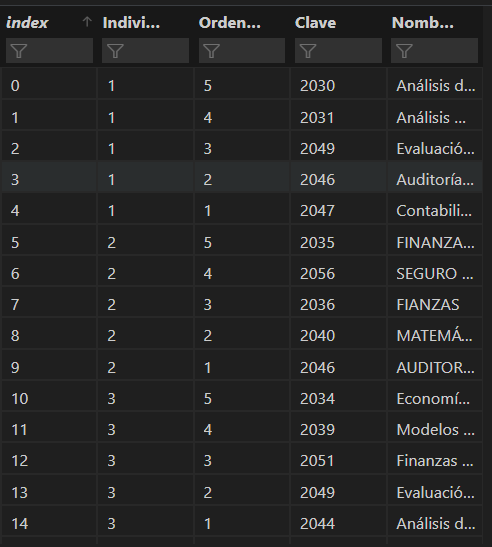
\includegraphics[scale=0.4]{Multimedia/Estructura_datos.png}
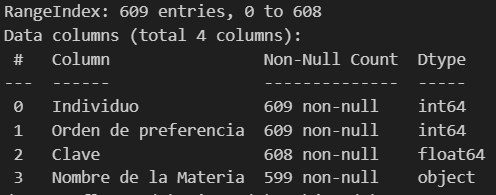
\includegraphics[scale=0.7]{Multimedia/Estructura_datos2.png}
\caption{Estructura de los datos}
\end{figure}

Las columnas de este conjunto de datos no son de utilidad para el análisis, por lo que de ellas solo nos interesa obtener el número de
elementos únicos que hay en cada una de ellas, llegando a los siguientes resultados:
% Lista con puntos como viñetas
\begin{itemize}
    \item \textbf{Estudiantes:} 124 elementos únicos
    \item \textbf{Materias:} 29 elementos únicos
\end{itemize}

Después de obtener el nivel de interes total que hay por materia se realiza un histograma de este interes y delimitamos una franja que en
el percentil del 25 por ciento, que marcará las materias a omitir si su interes está por debajo de este valor

\begin{figure}[H]
\centering
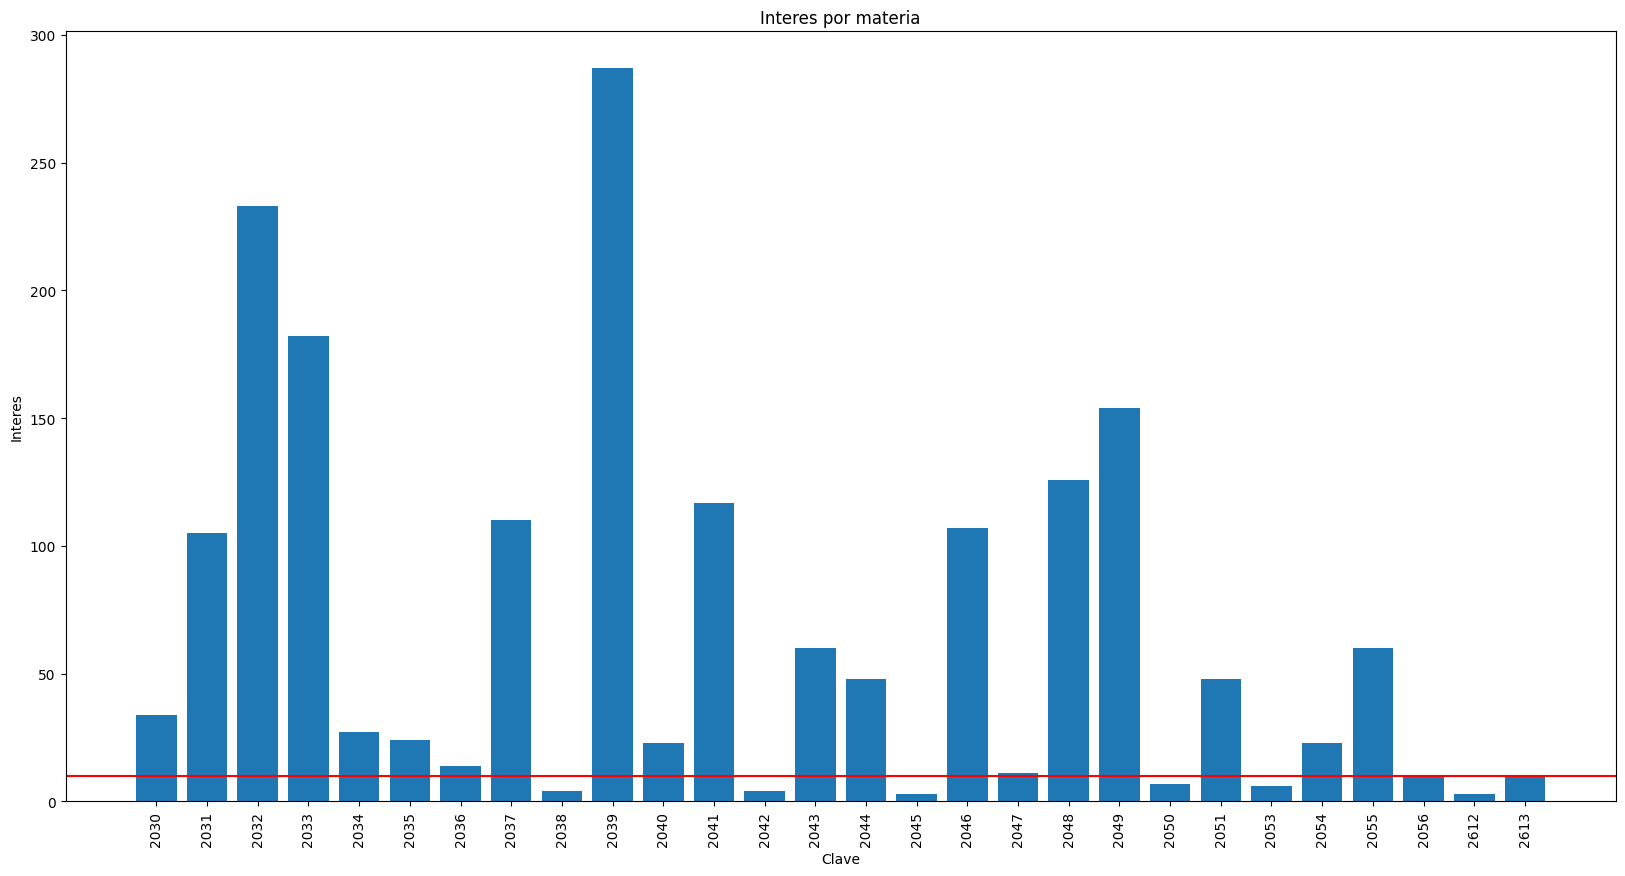
\includegraphics[scale=0.4]{Multimedia/hist_interes.png}
\caption{Histograma del interes por materia}
\end{figure}

Se adjunta además el análisis descriptivo de la variable de interes por materia:
\begin{figure}[H]
\centering
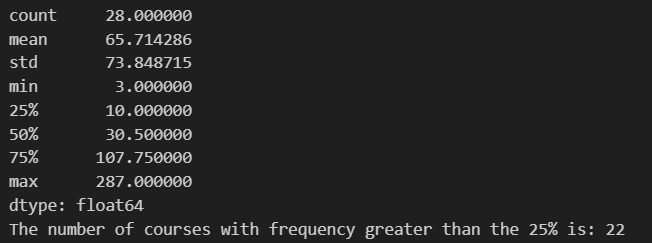
\includegraphics[scale=0.4]{Multimedia/Analisis_interes.png}
\caption{Análisis descriptivo de la variable de interes por materia}
\end{figure}

\newpage

\section{Análisis utilizando la técnica}

Se generó un dendo grama para visualizar los grupos que se formaron, obteniendo el siguiente resultado:
\begin{figure}[H]
\centering
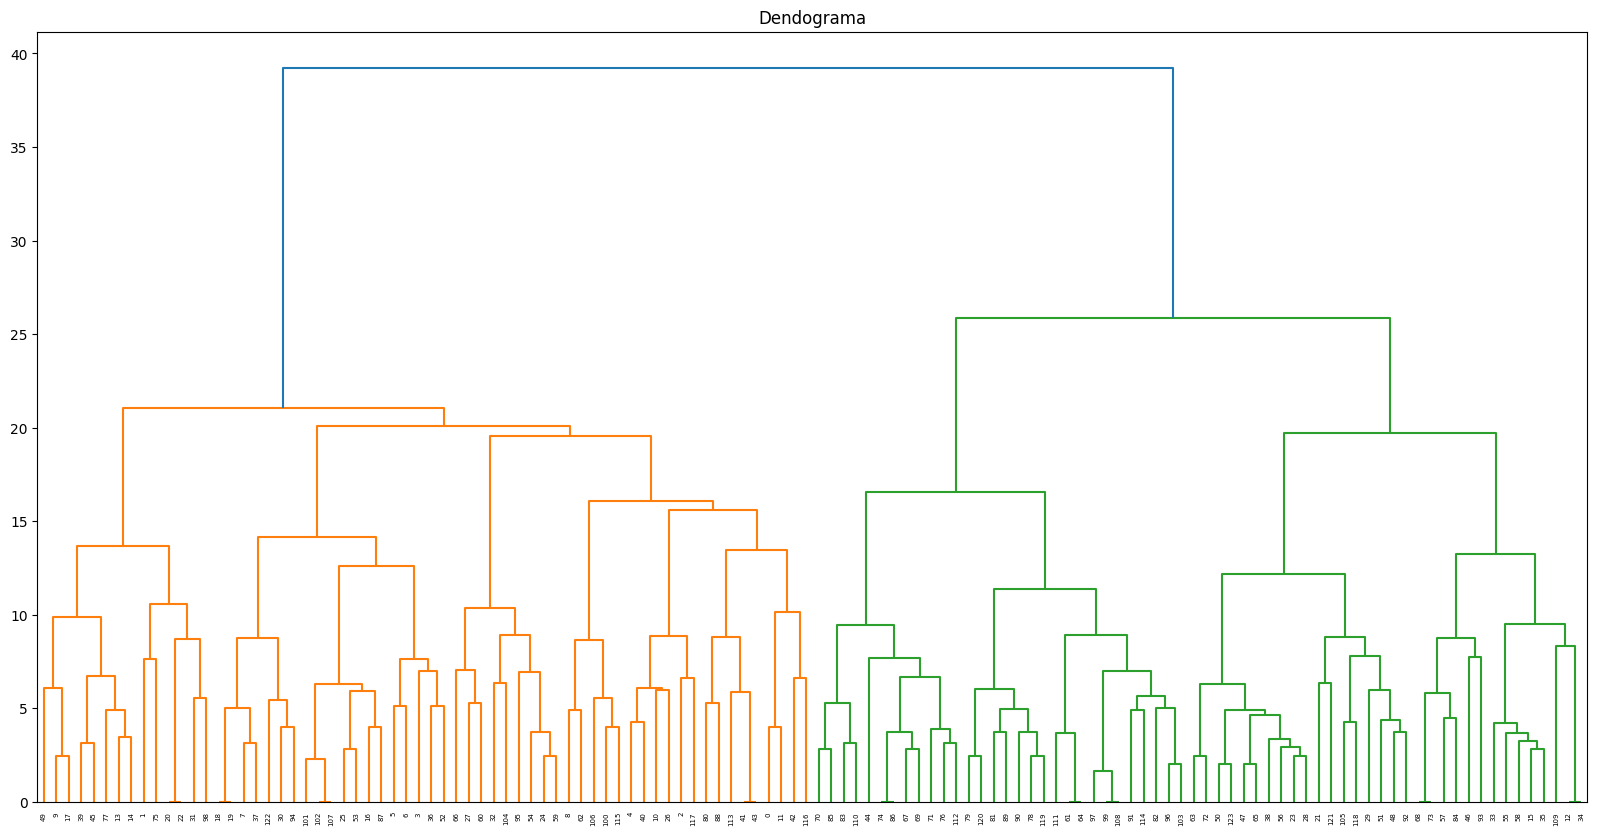
\includegraphics[scale=0.4]{Multimedia/Dendograma.png}
\caption{Dendograma}
\end{figure}

En este dendograma se puede observar que se formaron 2 grupos, ambos con muchos individuos, por lo que se decide realizar un análisis
mediante el método de k-means, con el fin de obtener un número de grupos más adecuado.\\

Se realizó un diagrama de codo para determinar el número óptimo de clusters, obteniendo el siguiente resultado:
\begin{figure}[H]
\centering
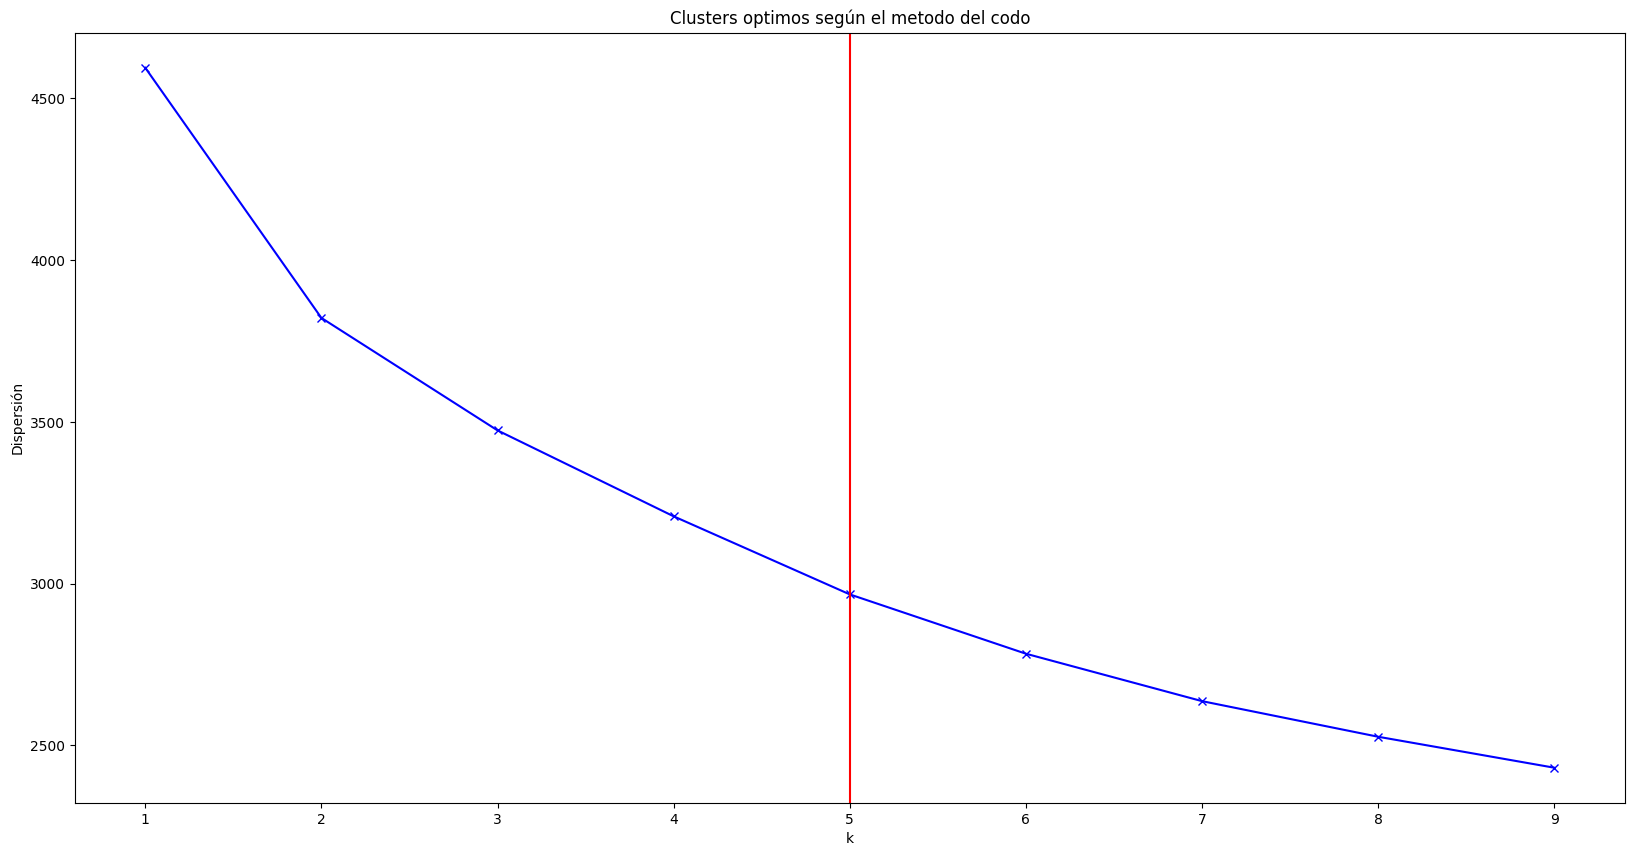
\includegraphics[scale=0.4]{Multimedia/Codo.png}
\caption{Diagrama de codo}
\end{figure}

El análisis mostró que por lo menos hasta la iteración 9 se siguen obteniendo mejoras en la suma de cuadrados, aunque la mejora respecto
a nuestra limitante de 5 grupos no es tan significativa, por lo que se decide tomar este número de grupos para el análisis.

\noindent Se realizó la agrupación de los datos, obteniendo los siguientes resultados:
\begin{figure}[H]
\centering
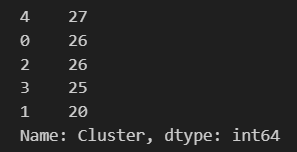
\includegraphics[scale=0.8]{Multimedia/Size_clusters.png}
\caption{Cantidad de alumnos en cada grupo}
\end{figure}

Mediante un análisis de los centroides de cada grupo, se determinaron las materias que se impartirán en cada grupo, formando
los siguientes grupos:

\begin{itemize}
    \item \textbf{Grupo 0:} Derivados, Evaluación de Proyectos, Auditoria Actuarial, Análisis Multivariado, Modelos y simulación
    \item \textbf{Grupo 1:} Investigación de Operaciones II, Análisis de Regresión, Modelos y simulación, Muestreo, Evaluación de Proyectos
    \item \textbf{Grupo 2:} Estadística Bayesiana, Muestreo, Modelos y simulación, Análisis de Regresión, Series de Tiempo
    \item \textbf{Grupo 3:} Auditoria Actuarial, Modelos y simulación, Planeación financiera, Evaluación de Proyectos, Análisis de estados financieros
    \item \textbf{Grupo 4:} Análisis de Regresión, Modelos y simulación, Análisis Multivariado, Derivados, Series de Tiempo
\end{itemize}

\section{Conclusión}

A lo largo del análisis se vió que hay gran variación en el interes que tienen los alumnos por las materias, lo que planteó múltiples
problemas a la hora de formar los grupos. Sin embargo, con el uso de técnicas estadísticas se logró formar grupos que puedan satisfacer
a la mayoría de los alumnos, reduciendo la inconformidad de los mismos.\\
Este análisis puede ser de gran utilidad para las autoridades de la facultad, ya que les permite formar grupos de manera más objetiva,
eficiente y con un menor grado de arbitrariedad, lo que puede contribuir a un aumento en el rendimiento académico de los alumnos.\\
Se debe resaltar que este análisis no es perfecto, ya que no se pueden satisfacer las necesidades de todos los alumnos retirando materias
que son de baja demanda\\
Se presupone que este análisis es fácilmente replicable para otros semestres, lo que ahorraría tiempo y esfuerzo a las autoridades de la
facultad.

\section{Bibliografía}

\begin{itemize}
    \item Herrera, M. (2023). \textit{Apuntes AR y AM}. Universidad Nacional Autónoma de México
    \item Microsoft Bing. (2023). Conversación personal sobre K-means.
    \item Towards Data Science. (24/10/2023). Understanding K-means Clustering in Machine Learning. Towards Data Science.
    Recuperado de \href[]{https://towardsdatascience.com/understanding-k-means-clustering-in-machine-learning-6a6e67336aa1}{Towards Data Science} 
\end{itemize}

\section{Anexo}

Para la realzación de este trabajo se modificó la base de datos original, la cual estaba llena de errores de captura principalmente
en los nombres de las materias.\\
Se removió la columna de ``Nombre de la materia'', además se removieron las filas que contenían datos faltantes.
Posteriormente se sustituyo los valores de ``2511'' por el valor de ``2037'' en la columna clave, ya que se trataba de un error de captura.\\
Posteriormente generé un dataframe con las veces que los alumnos eligieron cada materia, y el nivel de interes de las mismas.
\\
Luego, se formó un nuevo comnjunto de datos estableciendo la clave de las materias como columnas con el nivel de interes como valor.
Asimismo se definió al individuo como el índice de las filas y se removieron aquellas materias que tuvieran un nivel de interes menor
al del percentil 25.\\
Se adjunta el código utilizado para la limpieza de los datos y el análisis en el documento ``Análisis Optativas''.
\end{document}